%%%%%%%%%%%%%%%%%%%%%%%%%%%%%%%%%%%%%%%%%%%%%%%%%%%%%%%%%%
\frame {\frametitle{Functional Programming Roots}
%%%%%%%%%%%%%%%%%%%%%%%%%%%%%%%%%%%%%%%%%%%%%%%%%%%%%%%%%%
  \begin{itemize}
  \item \textbf{Key feature: higher order functions}
    \begin{itemize}
    \item Functions that accept other functions as arguments
    \item \textbf{Map} and \textbf{Fold}
    \end{itemize}
  \end{itemize}

  \begin{figure}[h]
    \centering
    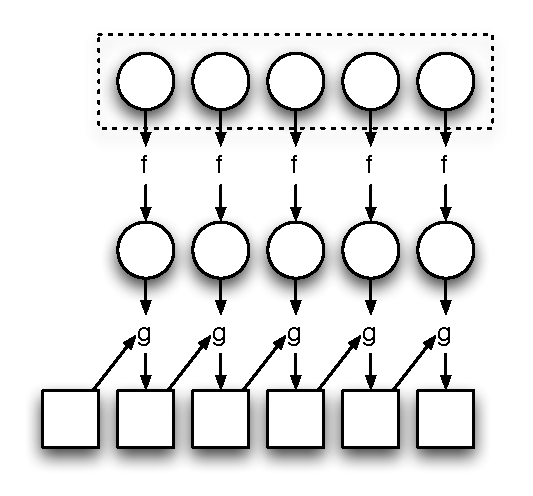
\includegraphics[scale=0.4]{./Figures/functional}
    \caption{Illustration of \emph{map} and \emph{fold}.}
    \label{fig:functional}
  \end{figure}
}

%%%%%%%%%%%%%%%%%%%%%%%%%%%%%%%%%%%%%%%%%%%%%%%%%%%%%%%%%%
\frame {\frametitle{Functional Programming Roots}
%%%%%%%%%%%%%%%%%%%%%%%%%%%%%%%%%%%%%%%%%%%%%%%%%%%%%%%%%%
  \begin{itemize}
  \item \textbf{map phase:}
    \begin{itemize}
    \item Given a list, \emph{map} takes as an argument a function $f$
      (that takes a single argument) and applies it to all element in a list
    \end{itemize}

    \vspace{20pt}

  \item \textbf{fold phase:}
    \begin{itemize}
    \item Given a list, fold takes as arguments a function $g$ (that
      takes two arguments) and an initial value (an accumulator)
    \item $g$ is first applied to the initial value and the first
      item in the list
    \item The result is stored in an intermediate variable, which is
      used as an input together with the next item to a second
      application of $g$
    \item The process is repeated until all items in the list have
      been consumed
    \end{itemize}
 \end{itemize}
}

%%%%%%%%%%%%%%%%%%%%%%%%%%%%%%%%%%%%%%%%%%%%%%%%%%%%%%%%%%
\frame {\frametitle{Functional Programming Roots}
%%%%%%%%%%%%%%%%%%%%%%%%%%%%%%%%%%%%%%%%%%%%%%%%%%%%%%%%%%
  \begin{itemize}
  \item \textbf{We can view map as a transformation over a dataset}
    \begin{itemize}
    \item This transformation is specified by the function $f$
    \item Each functional application happens in
      {\color{red} \textbf{isolation}}
    \item The application of $f$ to each element of a dataset can be
      parallelized in a straightforward manner
    \end{itemize}

    \vspace{20pt}

  \item \textbf{We can view fold as an aggregation operation}
    \begin{itemize}
    \item The aggregation is defined by the function $g$
    \item Data locality: elements in the list must be ``brought
      together''
    \item If we can {\color{red} \textbf{group}} elements of the list, also the fold phase can proceed in parallel 
    \end{itemize}

    \vspace{20pt}

  \item \textbf{Associative and commutative operations}
    \begin{itemize}
    \item Allow performance gains through local aggregation and reordering
    \end{itemize}
  \end{itemize}
 
}

%%%%%%%%%%%%%%%%%%%%%%%%%%%%%%%%%%%%%%%%%%%%%%%%%%%%%%%%%%
\frame {\frametitle{Functional Programming and MapReduce}
%%%%%%%%%%%%%%%%%%%%%%%%%%%%%%%%%%%%%%%%%%%%%%%%%%%%%%%%%%
  \begin{itemize}
  \item \textbf{Equivalence of MapReduce and Functional Programming: }
    \begin{itemize}
    \item The map of MapReduce corresponds to the map operation
    \item The reduce of MapReduce corresponds to the fold operation
    \end{itemize}

    \vspace{20pt}

  \item\textbf{The framework coordinates the map and reduce phases:}
    \begin{itemize}
    \item Grouping intermediate results happens in parallel
    \end{itemize}

    \vspace{20pt}
    
  \item \textbf{In practice:}
    \begin{itemize}
    \item User-specified computation is applied (in parallel) to all input
      records of a dataset
    \item Intermediate results are aggregated by another
      user-specified computation
    \end{itemize}

  \end{itemize}
}

%%%%%%%%%%%%%%%%%%%%%%%%%%%%%%%%%%%%%%%%%%%%%%%%%%%%%%%%%%
\frame {\frametitle{What can we do with MapReduce?}
%%%%%%%%%%%%%%%%%%%%%%%%%%%%%%%%%%%%%%%%%%%%%%%%%%%%%%%%%%
  \begin{itemize}
  \item \textbf{MapReduce ``implements'' a subset of functional
      programming}
    \begin{itemize}
    \item The programming model appears quite limited and strict
    \end{itemize}

\vspace{20pt}

  \item \textbf{There are several important problems that can be
      adapted to MapReduce}
    \begin{itemize}
    \item We will focus on illustrative cases
    \item We will see in detail ``design patterns''
      \begin{itemize}
      \item How to transform a problem and its input
      \item How to save memory and bandwidth in the system
      \end{itemize}
    \end{itemize}

  \end{itemize}

}

%%%%%%%%%%%%%%%%%%%%%%%%%%%%%%%%%%%%%%%%%%%%%%%%%%%%%%%%%%
\frame {\frametitle{Data Structures}
%%%%%%%%%%%%%%%%%%%%%%%%%%%%%%%%%%%%%%%%%%%%%%%%%%%%%%%%%%
  \begin{itemize}
  \item \textbf{Key-value pairs are the basic data structure in
      MapReduce}
    \begin{itemize}
    \item Keys and values can be: integers, float, strings, raw bytes
    \item They can also be \textbf{arbitrary data structures}
    \end{itemize}

    \vspace{20pt}

  \item \textbf{The design of MapReduce algorithms involves}:
    \begin{itemize}
    \item Imposing the key-value structure on arbitrary datasets\footnote{There's more about it: here we only look at the input to the map function.}
      \begin{itemize}
      \item E.g.: for a collection of Web pages, input keys may be URLs
        and values may be the HTML content
      \end{itemize}
    \item In some algorithms, input keys are not used, in others they
      uniquely identify a record
    \item Keys can be combined in complex ways to design various algorithms
    \end{itemize}
  \end{itemize}
}

%%%%%%%%%%%%%%%%%%%%%%%%%%%%%%%%%%%%%%%%%%%%%%%%%%%%%%%%%%
\frame {\frametitle{A Generic MapReduce Algorithm}
%%%%%%%%%%%%%%%%%%%%%%%%%%%%%%%%%%%%%%%%%%%%%%%%%%%%%%%%%%
  \begin{itemize}
  \item \textbf{The programmer defines a mapper and a reducer as
      follows}\footnote{We use the convention $[ \cdots ]$ to denote a list.}\footnote{Pedices indicate different data types.}:
    \begin{itemize}
    \item map: $(k_1,v_1) \to [(k_2,v_2)]$
    \item reduce: $(k_2,[v_2]) \to [(k_3,v_3)]$
    \end{itemize}

    \vspace{20pt}

  \item \textbf{In words}:
    \begin{itemize}
    \item A dataset stored on an underlying \textbf{distributed} filesystem,
      which is split in a number of \textbf{blocks} across machines
    \item The mapper is applied to every input key-value pair to
      generate intermediate key-value pairs
    \item The reducer is applied to all values associated with the
      same intermediate key to generate output key-value pairs
    \end{itemize}
  \end{itemize}
}

%%%%%%%%%%%%%%%%%%%%%%%%%%%%%%%%%%%%%%%%%%%%%%%%%%%%%%%%%%
\frame {\frametitle{Where the magic happens}
%%%%%%%%%%%%%%%%%%%%%%%%%%%%%%%%%%%%%%%%%%%%%%%%%%%%%%%%%%
  \begin{itemize}
  \item \textbf{Implicit between the map and reduce phases is a {\color{red}parallel ``\textbf{group by}''} operation on intermediate keys}
    \begin{itemize}
    \item Intermediate data arrive at each reducer in order, sorted by
      the key
    \item No ordering is guaranteed across reducers
   \end{itemize}

    \vspace{20pt}

  \item \textbf{Output keys from reducers are written back to the
      distributed filesystem}
    \begin{itemize}
    \item The output may consist of $r$ distinct files, where $r$ is
      the number of reducers
    \item Such output may be the input to a subsequent MapReduce phase\footnote{Think of \textbf{iterative algorithms}.}
    \end{itemize}

    \vspace{20pt}

  \item \textbf{Intermediate keys are transient}:
    \begin{itemize}
    \item They are not stored on the distributed filesystem
    \item They are ``spilled'' to the local disk of each machine in
      the cluster
    \end{itemize}
  \end{itemize}
}

%%%%%%%%%%%%%%%%%%%%%%%%%%%%%%%%%%%%%%%%%%%%%%%%%%%%%%%%%%
\frame {\frametitle{``Hello World'' in MapReduce}
%%%%%%%%%%%%%%%%%%%%%%%%%%%%%%%%%%%%%%%%%%%%%%%%%%%%%%%%%%

\begin{algorithm}[H]
\algrenewcommand\algorithmicfunction{\textbf{class}}
\algrenewcommand\algorithmicprocedure{\textbf{method}}

  \begin{algorithmic}[1]
    \Function{Mapper}{}
    \Procedure{Map}{offset $a$, line $l$}
    \ForAll{term $t \in$ line $l$}
      \State $\textsc{Emit}(\textrm{term }t, \textrm{count }1)$
    \EndFor
    \EndProcedure
    \EndFunction
  \end{algorithmic}
  
  \begin{algorithmic}[1]
    \Function{Reducer}{}
    \Procedure{Reduce}{term $t$, counts $[  c_1, c_2, \ldots ]$}
    \State $sum \gets 0$
    \ForAll{$ \textrm{count }c \in \textrm{counts }[  c_1, c_2, \ldots ]$}
    \State $sum \gets sum + c$
    \EndFor
    \State $\textsc{Emit}(\textrm{term }t, \textrm{count }sum)$
    \EndProcedure
    \EndFunction
  \end{algorithmic}

\end{algorithm}

}

%%%%%%%%%%%%%%%%%%%%%%%%%%%%%%%%%%%%%%%%%%%%%%%%%%%%%%%%%%
\frame {\frametitle{}
%%%%%%%%%%%%%%%%%%%%%%%%%%%%%%%%%%%%%%%%%%%%%%%%%%%%%%%%%%
  \begin{figure}[h]
    \centering
    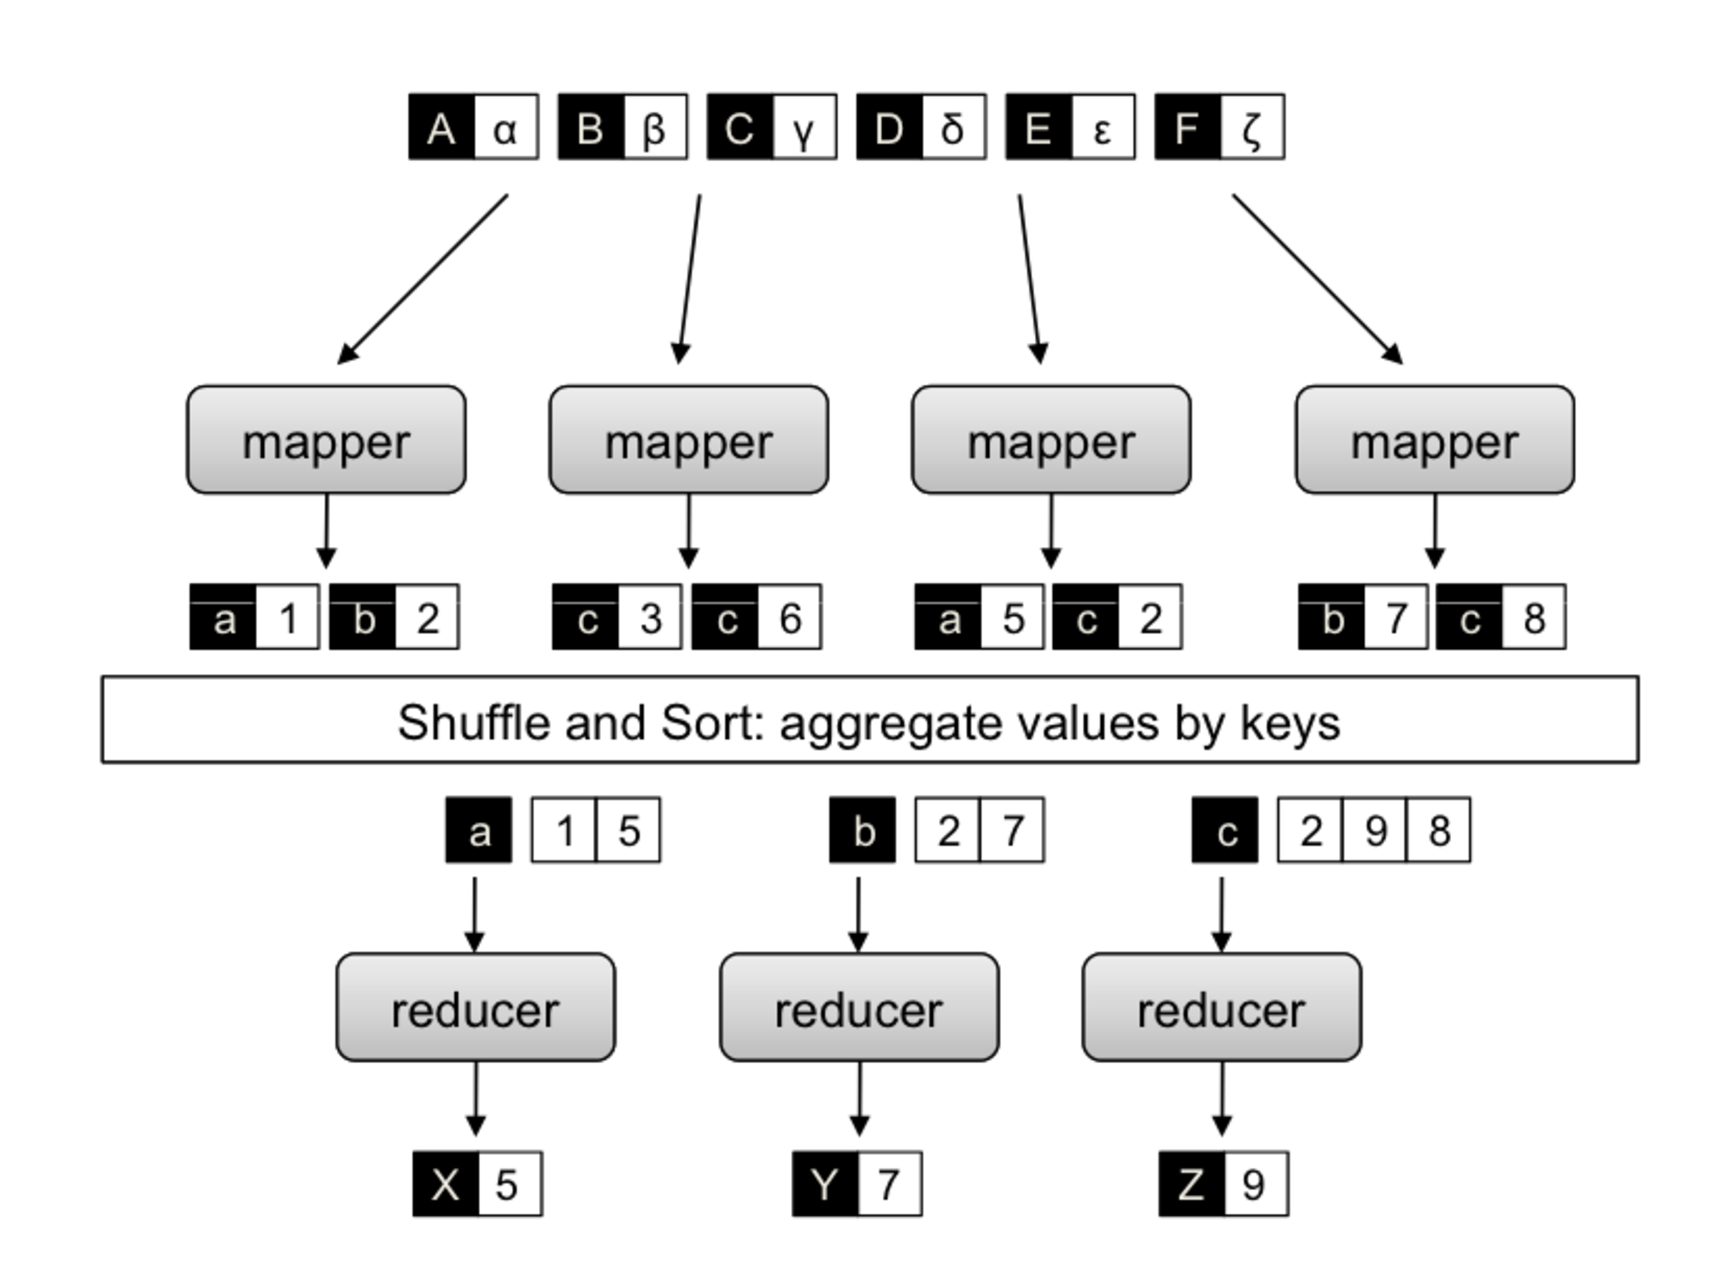
\includegraphics[scale=0.23]{./Figures/simple_MR}
    \label{fig:simple_MR}
  \end{figure}
}

\frame {\frametitle{``Hello World'' in MapReduce}
  \begin{itemize}

  \item \textbf{Input:}
    \begin{itemize}
    \item Key-value pairs: (offset, line) of a file stored on the distributed filesystem
    \item a: unique identifier of a line offset
    \item l: is the text of the line itself
    \end{itemize}

  \item \textbf{Mapper:}
    \begin{itemize}
    \item Takes an input key-value pair, tokenize the line 
    \item Emits intermediate key-value pairs: the word is the key and
      the integer is the value
    \end{itemize}

  \item \textbf{The framework:}
    \begin{itemize}
    \item Guarantees all values associated with the same key (the
      word) are brought to the same reducer
    \end{itemize}

  \item \textbf{The reducer:}
    \begin{itemize}
    \item Receives all values associated to some keys
    \item Sums the values and writes output key-value pairs: the key
      is the word and the value is the number of occurrences
    \end{itemize}
  \end{itemize}
}

%%%%%%%%%%%%%%%%%%%%%%%%%%%%%%%%%%%%%%%%%%%%%%%%%%%%%%%%%%
\frame {\frametitle{Combiners}
%%%%%%%%%%%%%%%%%%%%%%%%%%%%%%%%%%%%%%%%%%%%%%%%%%%%%%%%%%
  \begin{itemize}
  \item \textbf{Combiners are a general mechanism to reduce the amount
      of intermediate data}
    \begin{itemize}
    \item They could be thought of as ``mini-reducers''
    \end{itemize}

    \vspace{20pt}

  \item \textbf{Back to our running example: word count}
    \begin{itemize}
    \item Combiners aggregate term counts across documents processed
      by each map task
    \item If combiners take advantage of all opportunities for local
      aggregation we have at most $m \times V$ intermediate key-value
      pairs
      \begin{itemize}
      \item $m$: number of mappers
      \item $V$: number of unique terms in the collection
      \end{itemize}
    \item Note: due to Zipfian nature of term distributions, not all
      mappers will see all terms
    \end{itemize}
    
  \end{itemize}
}

%%%%%%%%%%%%%%%%%%%%%%%%%%%%%%%%%%%%%%%%%%%%%%%%%%%%%%%%%%
\frame {\frametitle{A word of caution}
%%%%%%%%%%%%%%%%%%%%%%%%%%%%%%%%%%%%%%%%%%%%%%%%%%%%%%%%%%
  \begin{itemize}
  \item \textbf{The use of combiners must be thought carefully}
    \begin{itemize}
    \item In Hadoop, they are optional: the correctness of the
      algorithm cannot depend on computation (or even execution) of
      the combiners
    \end{itemize}

    \vspace{20pt}

  \item \textbf{Combiners I/O types}
    \begin{itemize}
    \item Input: $(k_2, [v_2])$ [Same input as for Reducers]
    \item Output: $[(k_2, v_2)]$ [Same output as for Mappers]
    \end{itemize}

    \vspace{20pt}

  \item \textbf{Commutative and Associative computations}
    \begin{itemize}
    \item Reducer and Combiner code may be interchangeable (e.g. Word Count)
    \item This is not true in the general case
    \end{itemize}
  \end{itemize}
}

%%%%%%%%%%%%%%%%%%%%%%%%%%%%%%%%%%%%%%%%%%%%%%%%%%%%%%%%%%
\frame {\frametitle{}
%%%%%%%%%%%%%%%%%%%%%%%%%%%%%%%%%%%%%%%%%%%%%%%%%%%%%%%%%%
   \begin{center}
   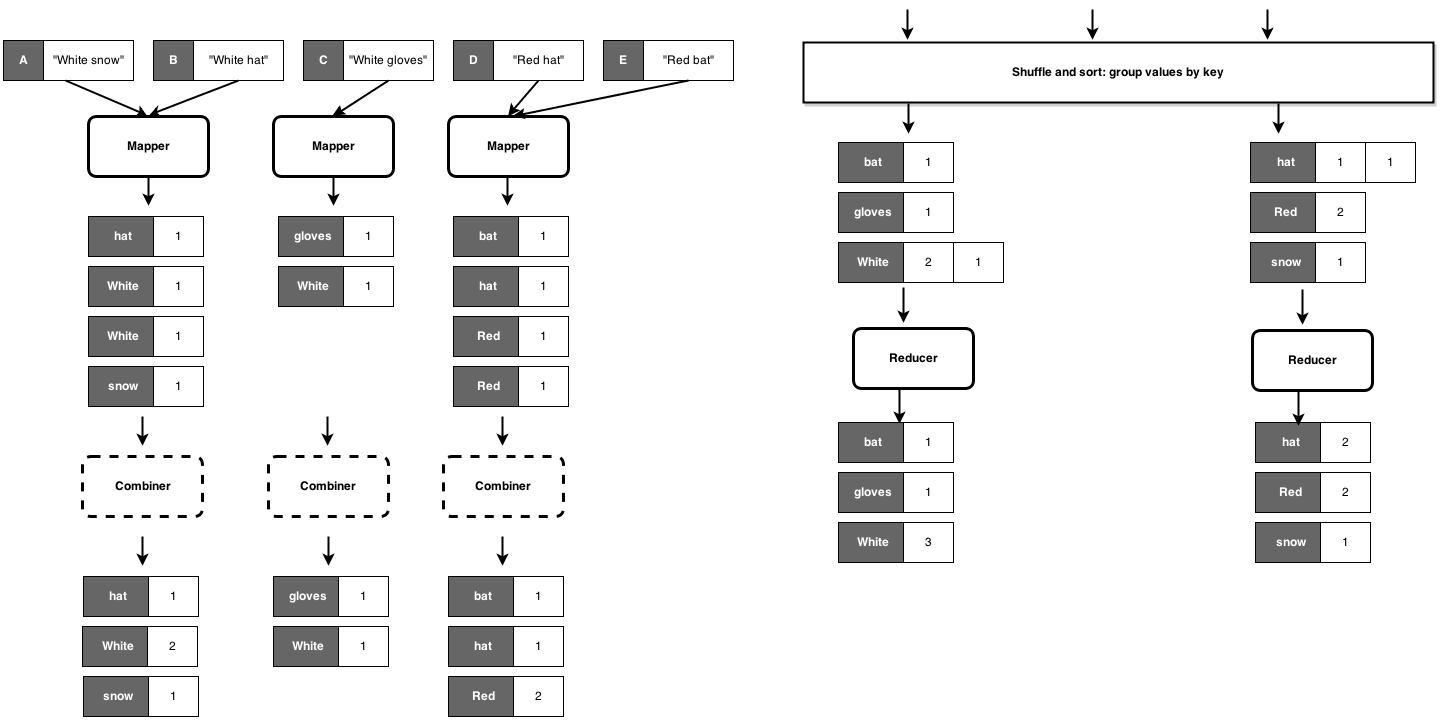
\includegraphics[scale=0.23]{./Figures/simple_MR_combiners}
    \end{center}
}



%%%%%%%%%%%%%%%%%%%%%%%%%%%%%%%%%%%%%%%%%%%%%%%%%%%%%%%%%%
\frame {\frametitle{Algorithmic Correctness: an Example}
%%%%%%%%%%%%%%%%%%%%%%%%%%%%%%%%%%%%%%%%%%%%%%%%%%%%%%%%%%
  \begin{itemize}
  \item \textbf{Problem statement}
    \begin{itemize}
    \item We have a large dataset where input keys are strings and input
      values are integers
    \item We wish to compute the mean of all integers associated with
      the same key
      \begin{itemize}
      \item In practice: the dataset can be a log from a website,
        where the keys are user IDs and values are some measure of activity
      \end{itemize}
    \end{itemize}

    \vspace{20pt}

  \item \textbf{Next, a baseline approach}
    \begin{itemize}
    \item We use an \textbf{identity mapper}, which groups and sorts
      appropriately input key-value pairs
    \item Reducers keep track of running sum and the number of
      integers encountered
    \item The mean is emitted as the output of the reducer, with the
      input string as the key
    \end{itemize}

    \vspace{20pt}

  \item \textbf{Inefficiency problems in the shuffle phase}
  \end{itemize}
}

%%%%%%%%%%%%%%%%%%%%%%%%%%%%%%%%%%%%%%%%%%%%%%%%%%%%%%%%%%
\frame {\frametitle{Example: Computing the mean}
%%%%%%%%%%%%%%%%%%%%%%%%%%%%%%%%%%%%%%%%%%%%%%%%%%%%%%%%%%
\begin{algorithm}[H]
\algrenewcommand\algorithmicfunction{\textbf{class}}
\algrenewcommand\algorithmicprocedure{\textbf{method}}
  \begin{algorithmic}[1]
    \Function{Mapper}{}
    \Procedure{Map}{string $t$, integer $r$}
    \State $\textsc{Emit}(\textrm{string }t, \textrm{integer }r)$
    \EndProcedure
    \EndFunction
  \end{algorithmic}

  \begin{algorithmic}[1]
    \Function{Reducer}{}
    \Procedure{Reduce}{string $t$, integers $[ r_1, r_2, \ldots ]$}
    \State $sum \gets 0$
    \State $cnt \gets 0$
    \ForAll{$ \textrm{integer }r \in \textrm{integers }[ r_1, r_2, \ldots ]$}
    \State $sum \gets sum + r$
    \State $cnt \gets cnt + 1$
    \EndFor
    \State $r_{avg} \gets sum/cnt$
    \State $\textsc{Emit}(\textrm{string }t, \textrm{integer } r_{avg})$
    \EndProcedure
    \EndFunction
  \end{algorithmic}
\end{algorithm}
}

%%%%%%%%%%%%%%%%%%%%%%%%%%%%%%%%%%%%%%%%%%%%%%%%%%%%%%%%%%
\frame {\frametitle{Algorithmic Correctness}
%%%%%%%%%%%%%%%%%%%%%%%%%%%%%%%%%%%%%%%%%%%%%%%%%%%%%%%%%%
  \begin{itemize}
  \item \textbf{Note: operations are not distributive}
    \begin{itemize}
    \item \texttt{Mean}(1,2,3,4,5) $\neq$
      \texttt{Mean}(\texttt{Mean}(1,2), \texttt{Mean}(3,4,5))
    \item Hence: a combiner cannot output partial means and hope that
      the reducer will compute the correct final mean
    \end{itemize}

    \vspace{20pt}

  \item \textbf{Rule of thumb:}
    \begin{itemize}
      \item Combiners are optimizations, the algorithm should work even when ``removing'' them
    \end{itemize}   
  \end{itemize}
}

%%%%%%%%%%%%%%%%%%%%%%%%%%%%%%%%%%%%%%%%%%%%%%%%%%%%%%%%%%
\frame {\frametitle{Example: Computing the mean with combiners}
%%%%%%%%%%%%%%%%%%%%%%%%%%%%%%%%%%%%%%%%%%%%%%%%%%%%%%%%%%

\begin{algorithm}[H]
\algrenewcommand\algorithmicfunction{\textbf{class}}
\algrenewcommand\algorithmicprocedure{\textbf{method}}
\begin{tiny}
  \begin{algorithmic}[1]
    \Function{Mapper}{}
    \Procedure{Map}{string $t$, integer $r$}
    \State $\textsc{Emit}(\textrm{string }t, \textrm{pair }(r, 1))$
    \EndProcedure
    \EndFunction
  \end{algorithmic}

  \begin{algorithmic}[1]
    \Function{Combiner}{}
    \Procedure{Combine}{string $t$, pairs $[ (s_1, c_1), (s_2, c_2) \ldots ]$}
    \State $sum \gets 0$
    \State $cnt \gets 0$
    \ForAll{$ \textrm{pair }(s, c) \in \textrm{pairs }[ (s_1, c_1), (s_2, c_2) \ldots ]$}
    \State $sum \gets sum + s$
    \State $cnt \gets cnt + c$
    \EndFor
    \State $\textsc{Emit}(\textrm{string }t, \textrm{pair }(sum, cnt))$
    \EndProcedure
    \EndFunction
  \end{algorithmic}

  \begin{algorithmic}[1]
    \Function{Reducer}{}
    \Procedure{Reduce}{string $t$, pairs $[ (s_1, c_1), (s_2, c_2) \ldots ]$}
    \State $sum \gets 0$
    \State $cnt \gets 0$
    \ForAll{$ \textrm{pair }(s, c) \in \textrm{pairs }[ (s_1, c_1), (s_2, c_2) \ldots ]$}
    \State $sum \gets sum + s$
    \State $cnt \gets cnt + c$
    \EndFor
    \State $r_{avg} \gets sum/cnt$
    \State $\textsc{Emit}(\textrm{string }t, \textrm{integer } r_{avg})$
    \EndProcedure
    \EndFunction
  \end{algorithmic}
\end{tiny}
\end{algorithm}

}

